\subsection{Ingestion}

As a primary data source for the use case of Air traffic monitoring, \href{https://www.satori.com/}{Satori} and its air traffic channel have been chosen given the easy to use APIs made available to connect to the data stream. Satori is a portal where organizations can publish their open data and offers a wide variety of channels, that is data endpoints, to be used: from transportation channels, to weather related channels. The \href{https://www.satori.com/channels/air-traffic}{air-traffic channel} republishes data from \href{https://planefinder.net/}{Planefinder}, filtering only aircrafts above 37000 feet of altitude, effectively cutting most of national flights which don't even reach that altitude. In a real world application on air traffic monitoring, it would be necessary to use more than a single data source, additionally using commercial data services such as \href{http://flightaware.com/}{FlightAware} and \href{http://flightradar24.com/}{FlightRadar24} in order to get the most information available.
\\\\
Data Ingestion's pipeline is composed of 2 main components: NiFi, handling distributed execution of the script used to connect to Satori and publishing the data to Kafka, which, in turn, handles the queueing and the serving to consumer applications (which is, in this case, a Flink Job).

JSON records ingested from Satori contain the following fields:

\begin{itemize}
    \item \textbf{origin}: IATA code of the airport from which the airplane has taken off;
    \item \textbf{destination}: IATA code of the airport to which the airplane will arrive;
    \item \textbf{aircraft}: model of the aircraft which has transmitted the current record
    \item \textbf{flight}: public code representing the airplane route
    \item \textbf{registration}: unique ICAAO identification for the aircraft which has transmitted the current record    
    \item \textbf{callsign}: radar-only code representing the airplane route
    \item \textbf{lat}: latitude
    \item \textbf{lon}: longitude
    \item \textbf{speed}: speed in Knots from the current record
    \item \textbf{altitude}: altitude in feet from the current record
    \item \textbf{course}: vector direction in degrees, measured clockwise from north (0°)
    \item \textbf{time}: timestamp since UNIX epoch in seconds of the current record
\end{itemize}

The ingestion pipeline in NiFi uses in total 4 Processors, as shown in \ref{fig:nifipipeline}. The first Processor used is \textbf{ExecuteProcess}, which is used to execute a Python script which connects to Satori through their already mentioned APIs and printing all of the fetched records, as lines containing Json Arrays, on the standard output. The flow continues then in the \textbf{SplitText} and \textbf{SplitJson} which, respectively, deal with singling out each Json Array and then extracting each Json Object, which is the actual record, to be then published on Kafka via the proper \textbf{PublishKafkaRecord\_0\_10} Processor.

\begin{figure}[ph]
    \centering
    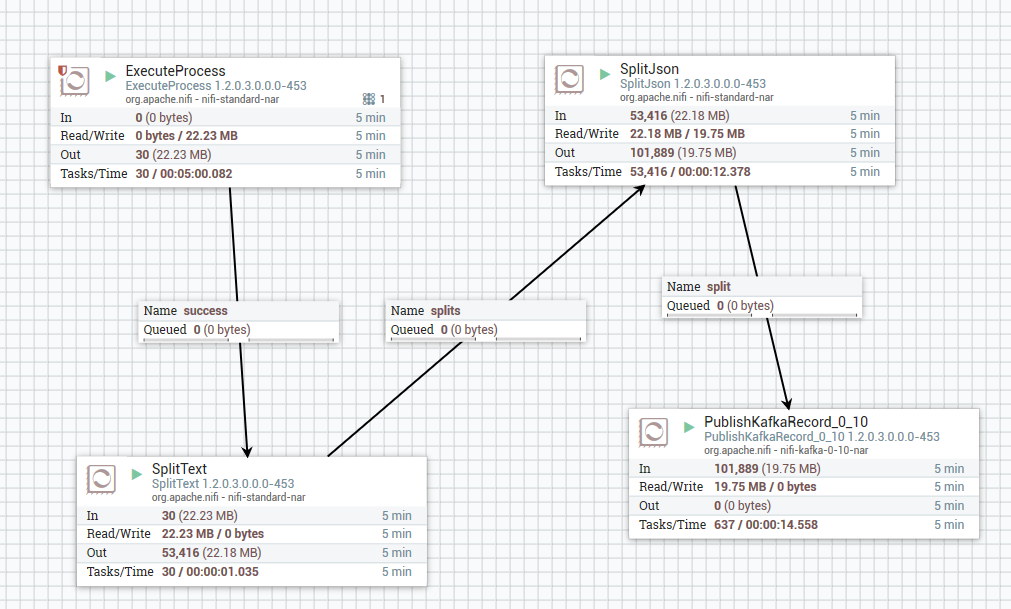
\includegraphics[width=0.7\linewidth]{Figures/nifipipeline}
    \caption{NiFi pipeline used for the ingestion from Satori}
    \label{fig:nifipipeline}
\end{figure}

In order to get into more details, let's list the entire pipeline:

\begin{enumerate}
    \item \textbf{ExecuteProcess} Processor, where the data fetching actually happens, it runs continuously the following script:
    
    \begin{code}
        \begin{minted}{Python}
with make_client(endpoint=endpoint, appkey=appkey) as client:
    
    class SubscriptionObserver(object):
        def on_subscription_data(self, data):
            for in_message in data['messages']:
                if all(len(str(x)) > 0 for x in in_message.values()):
                    fetched_data.append(json.dumps(in_message))
            got_message_event.set()
            
    subscription_observer = SubscriptionObserver()
    client.subscribe(
            "air-traffic",
            SubscriptionMode.SIMPLE,
            subscription_observer)
    
    while got_message_event.wait(10):
        if len(fetched_data) != 0:
            print(fetched_data)
     
        \end{minted}
    \end{code}
which basically uses Satori APIs to create a client subscribing to the Air Traffic JSON stream, fetching batches of JSON records, filtering those with empty values and printing each batch on standard output as a JSON array. ExecuteProcess will then create a \textbf{FlowFile} containing as a payload many JSON arrays from subsequent script calls, which will be the input for the following Processor;

\item \textbf{SplitText} simply deals with splitting a single FlowFile, with many JSON arrays, into that many FlowFiles containing only a single JSON array;
\item \textbf{SplitJson}, instead, deals with extracting all of the JSON Objects from the input JSON arrays, generating a FlowFile for each one of them;
\item \textbf{PublishKafkaRecord\_0\_10} is the NiFi Processor which publishes the incoming FlowFiles to a Kafka topic. Its required configuration needs the usual Kafka Producer settings: the broker list, a comma separated list of the broker listeners, in this case \texttt{master-1.localdomain:9092,master-2.localdomain:9092}, the topic in which each record needs to be published, \texttt{air\_traffic} and the security protocol used to publish, \texttt{PLAINTEXT}. Other than these settings, this Processor needs two components: a \textbf{Record Reader}, needed to deserialize the incoming FlowFiles, and a \textbf{Record Writer}, used to serialize each record before publishing it on Kafka. Said components are services provided by an \textbf{HortonworksSchemaRegistry}, a registry used to store Avro schemas\footnote{\textbf{\href{https://avro.apache.org/}{Avro}} is a data serialization system allowing to define types and possible values for JSON encoded records.} against which incoming records are validated to make sure they follow the specified schema. If validation succeeds, the record is then correctly published on the \texttt{air\_traffic} topic, serialized following the validated Avro schema.
\end{enumerate}

Data ingestion continues, then, in Kafka. As previously mentioned, a single topic called \texttt{air\_traffic} is used, configured with a retention time of 24 hours, a single partition, since throughput is approximately of $20000$ records per minute, accounting to 4 MB per minute, being a relatively sparse stream, and two replicas handled by both the active Kafka brokers.
\pagebreak